\documentclass[a4paper,14pt]{extarticle}

\usepackage[utf8]{inputenc}
\usepackage[english,russian]{babel}
\usepackage{listings}
\usepackage{caption}
\usepackage{indentfirst}
\usepackage{pdfpages} % Вставка PDF
\usepackage{float}

\usepackage{mathptmx}
\usepackage{graphicx}
\graphicspath{{images/}}

\renewcommand{\baselinestretch}{1.5}
\parindent 1cm % Абзацный отступ

\usepackage{geometry}
\geometry{left=3cm}
\geometry{right=1cm}
\geometry{top=2cm}
\geometry{bottom=2cm}

\usepackage{enumitem}
\setlist[enumerate,itemize]{leftmargin=12.7mm}
\makeatletter
    \AddEnumerateCounter{\asbuk}{\@asbuk}{м)}
\makeatother
\setlist{nolistsep} % Нет отступов между пунктами списка
\renewcommand{\labelitemi}{--} % Маркет списка --
\renewcommand{\labelenumi}{\asbuk{enumi})} % Список второго уровня
\renewcommand{\labelenumii}{\arabic{enumii})} % Список третьего уровня

\begin{document}
\begin{titlepage}
    \begin{center}
        Гайд по сборке GBot-tiny
    \end{center}
    
    \begin{figure}[H]
        \centering
        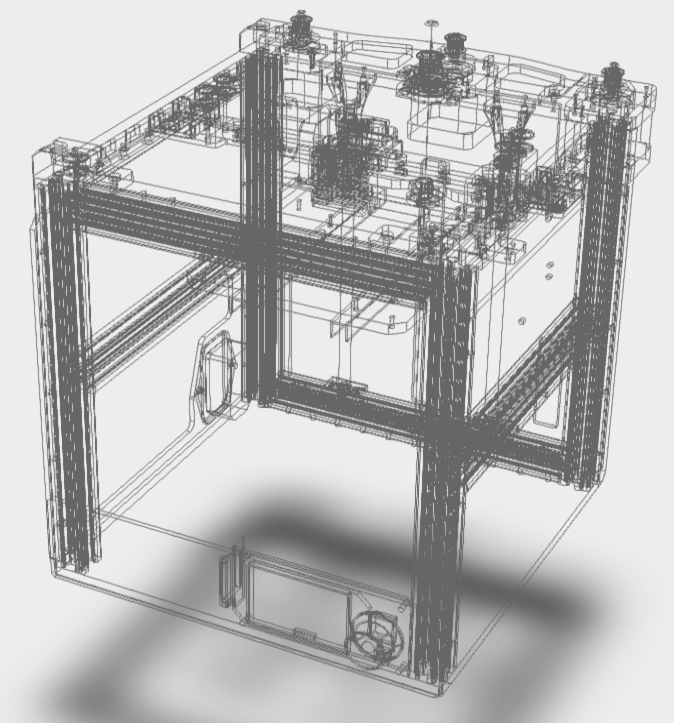
\includegraphics[width=\textwidth]{GBot-Tiny-preview}
        \label{gbot-tiny-preview}
    \end{figure}
    
\end{titlepage}

\tableofcontents
\clearpage

\section*{Введение}

Вводное слово

3д печатные части. и их рекомендации

Обратная связь

\clearpage

\section*{Материалы(BOM)}



\clearpage
\input{chapters/2-chapter}
\input{chapters/3-chapter}
\input{chapters/4-conclusion}


\end{document}